% =======================================================================
\section{Testing for Failures Refinement -- an Example}
\label{sec:case}
% =======================================================================

Generating the test cases $U_F(p)$ specified in  (\ref{eq:UFP}) for the reference
process $P$ discussed in Example~\ref{example:CSP},
results in the   instantiations of initials, minimal hitting sets, and
transition function shown in Fig.~\ref{fig:initialsminhitstrans};
this can be directly derived from $P$'s normalised
transition graph with nodes $N =\{0,1,2,3\}$ displayed in Fig.~\ref{fig:tga}.

\begin{figure}[ht]
\footnotesize
\begin{center}
\begin{minipage}{0.2\textwidth}
	 \begin{eqnarray*}
{ }[0]^0 & = & \{ a \} \\
{ }[1]^0 & = & \{ a,b,c \} \\
{ }[2]^0 & = & \{ a,b,c \} \\
{ }[3]^0 & = & \{ b,c \}
\end{eqnarray*}
	\end{minipage}
	\hfill
	\begin{minipage}{0.33\textwidth}
	 \begin{eqnarray*}
\minhits(0) & = & \{ \{ a\} \} \\
\minhits(1) & = & \{ \{a,b\}, \{c\} \} \\
\minhits(2) & = & \{  \{a,b\},  \{a,c\}\} \\
\minhits(3) & = & \{ \{ b\}, \{c\} \}
\end{eqnarray*}

	\end{minipage}
	\hfill
	\begin{minipage}{0.2\textwidth}
	 \begin{eqnarray*}
t(0,a) & = & 1 \\
t(1,a) & = & 0 \\
t(1,b) & = & 0 \\
t(1,c) & = & 2
\end{eqnarray*}
	\end{minipage}
		\hfill
	\begin{minipage}{0.2\textwidth}
	 \begin{eqnarray*}
t(2,a) & = & 1 \\
t(2,b) & = & 0 \\
t(2,c) & = & 3 \\
t(3,b) & = & 0 \\
t(3,c) &  =& 3
\end{eqnarray*}
	\end{minipage}
\caption{Initials, minimal hitting sets, and transition function of the normalised transition graph displayed in Fig.~\ref{fig:tga}.}
\label{fig:initialsminhitstrans}
\end{center}
\normalsize
\end{figure}

% .....................................................................................
 \begin{figure}
 %%\hspace*{-40mm}
 \begin{center}
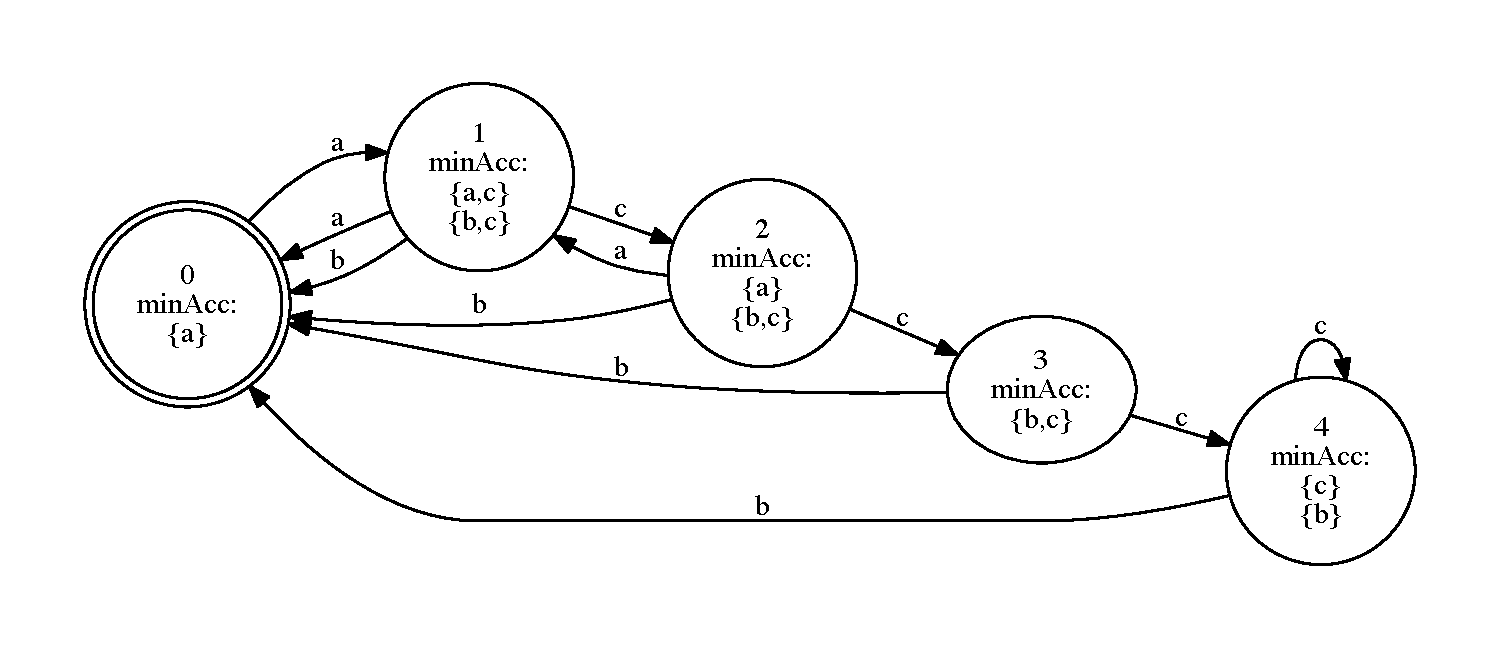
\includegraphics[trim=0cm 1.4cm 0cm 1.4cm,clip,scale=.6,%width=\textwidth
                 ]{z.pdf}
\end{center}
%%\vspace*{-10mm}
\caption{Normalised transition graph of faulty implementation $Z$  from Example~\ref{ex:uf1tests}.}
 \label{fig:tgZ}
 \end{figure}
% .......................................................................................

\begin{example}
\label{ex:uf1tests} Consider the following implementation $Z$ of process $P$
from Example~\ref{example:CSP} that is erroneous from the point of view of
failures refinement. In the specification of $Z$, it is assumed that $r_{max}\ge 0$.
\begin{eqnarray*}
  Z & = & a \then (Q_1 \intchoice R_1(r_{max},0))
  \\
  Q_1 & = & a\then Z \extchoice c\then Z
  \\
  R_1(r_{max},k) & = & (k < r_{max}) \& \big(b\then Z \extchoice  c\then R_1(r_{max},k+1)\big)
  \\ & & \extchoice
  \\ & & (k = r_{max}) \& \big(b\then Z \intchoice c\then R_1(r_{max},r_{max})\big)
\end{eqnarray*}
It can be checked with FDR that $Z$ is trace-equivalent to $P$. While $k <
r_{max}$, $Z$ also accepts the same sets of events as $P$. When
$R_1(r_{max},k)$ runs through several recursions and $k = r_{max}$, however,
$R_1(r_{max},k)$ makes an internal choice, instead of offering an external
choice, so $P\not\lessdet_F Z$. Fig.~\ref{fig:tgZ} shows the normalised
transition graph of $Z$ for $r_{max} = 3$.

Running the test $U_F(j)$ against $Z$ for $j=0,\dots,19$ ($G(P)$ has $p = 4$
states and $G(Z)$ has $q=5$, so $pq-1=19$ is the index of the last test to
be executed  according to Theorem~\ref{th:failurestest}), tests $U_F(0),\dots,
U_F(3)$ are passed by $Z$, but $Z$ fails $U_F(4)$, because after execution of
the trace
\[
s = a.c.c.c, \qquad\text{(note that $G(P)/s = \text{node}\ 3$ according to Fig.~\ref{fig:tga})},
\]
the test $U_F(4)$ offers hitting sets from $\minhits(3) = \{\{b\},\{c\}\}$
in branch (\ref{eq:ufd}). Therefore,  there exists one test execution
where $Z/s$ accepts only $\{b\}$ due to the internal choice (note
from Fig.~\ref{fig:tgZ} that
$G(Z)/s = \text{node}\ 4$), while $U_F(4)/s$
only offers $\{c\}$ in branch (\ref{eq:ufd}) or $\{ a\} = \Sigma - [3]^0$ for
branch (\ref{eq:ufa}).  As a consequence, this execution of
$(Z\parallel[\Sigma] U_F(4))/s$ deadlocks, and the $pass$ event cannot be
produced. Another failing execution arises if $Z/s$ chooses to accept only
$\{c \}$, while $U_F(4)/s$ choses to accept only $\{a,b\}$. Therefore,
$%\[
(\epass\then \Stop)\not\lessdet_F  (Z\parallel[\Sigma] U_F(4)) \hide\Sigma,
$ %\]
and the test fails. \xbox
\end{example}

% ======================================================================
